\documentclass{article}

% Language setting
% Replace `english' with e.g. `spanish' to change the document language
\usepackage[english]{babel}

% Set page size and margins
% Replace `letterpaper' with `a4paper' for UK/EU standard size
\usepackage[letterpaper,top=2cm,bottom=2cm,left=3cm,right=3cm,marginparwidth=1.75cm]{geometry}

% Useful packages
\usepackage{amsmath}
\usepackage{graphicx}
\usepackage[colorlinks=true, allcolors=blue]{hyperref}
\usepackage{pdfpages}
\usepackage{listings}
\usepackage{algorithm}
\usepackage{enumitem}
\usepackage{algpseudocode}
\usepackage{amssymb}

\title{Algorithmische Geometrie H13}
\author{Eli Kogan-Wang (7251030), Bogdan Rerich (7248483)}

\def\O{\mathcal{O}}

\begin{document}
%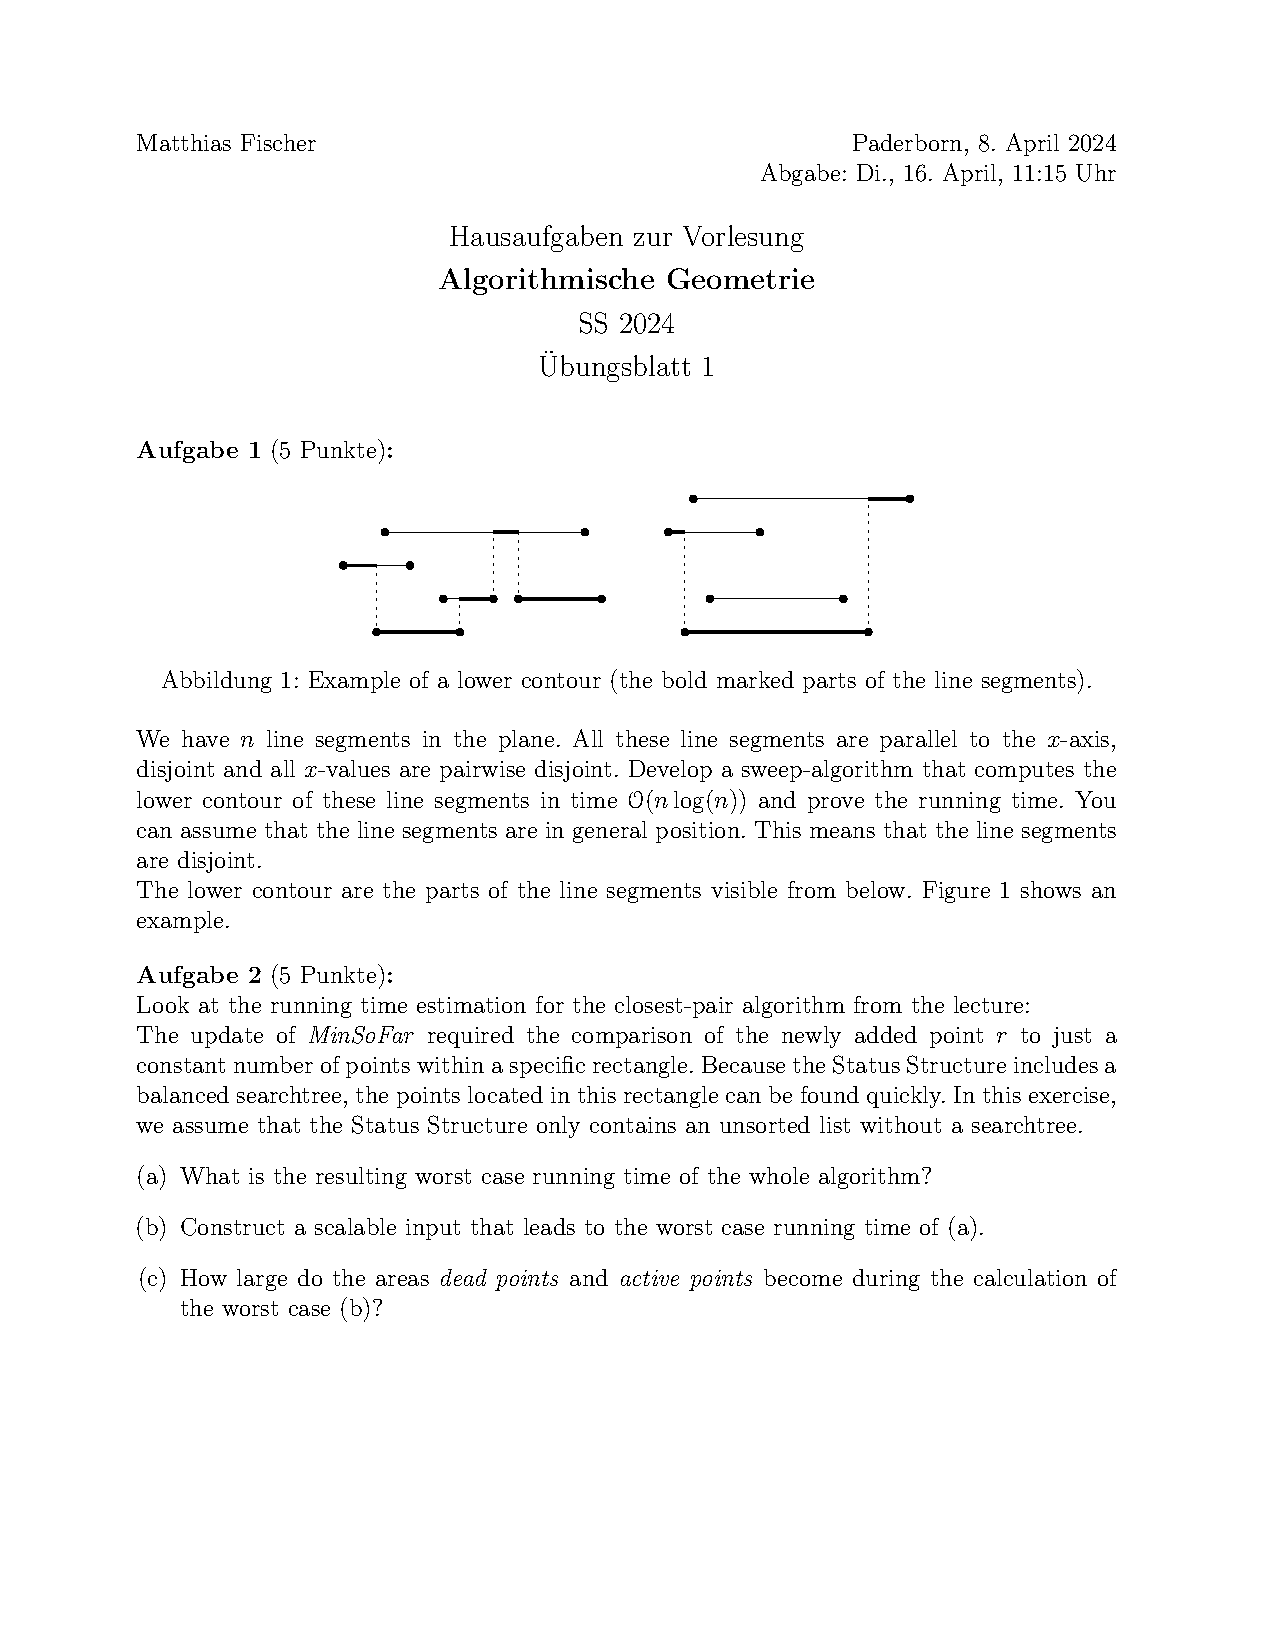
\includepdf[]{Blatt01.pdf}
\maketitle

% Matthias Fischer Paderborn, 3. Juli 2024
% Abgabe: Di., 16. Juli, 11:15 Uhr
% Hausaufgaben zur Vorlesung
% Algorithmische Geometrie
% SS 2024
% Übungsblatt 13
% Aufgabe 24 (5 Punkte):
% Prove that the smallest angle of any triangulation of a simple polygon whose vertices lie on a circle
% is the same.
% This implies that any completion of the Delaunay triangulation of a set of points which are not in
% general position (Delaunay decomposition), maximizes the minimum angle.

\textbf{Aufgabe 24 (5 Punkte):}

Let $S=\{p_1, p_2, \ldots, p_n\}$ be a set of points in the plane which lie on a circle.
We shall prove that the smallest angle of any triangulation of the convex hull of $S$ is the same.

Take $i$, such that $\|p_i - p_{i+1}\| = \min_{1 \leq j \leq n} \|p_j - p_{j+1}\|$, where $p_{n+1} = p_1$.
This means that the distance between $p_i$ and $p_{i+1}$ is the smallest among all distances between consecutive points.

It is also known, that any triangulation of a set of points includes all the edges of the convex hull of the set.
This means that $p_i$ and $p_{i+1}$ are connected by an edge in any triangulation of the convex hull of $S$.

Since a triangulation consists of triangles, there exists a vertex $p_j$ of a triangle, such that $p_i$, $p_{i+1}$ and $p_j$ are vertices of the same triangle.
Since $p_j$ is a vertex on the same circle as $p_i$ and $p_{i+1}$, the angle $\angle p_i p_j p_{i+1}$ is constant for all $j$.
% The inscribed angle theorem appears as Proposition 20 on Book 3 of Euclid's Elements.
This is because the angle subtended by a chord on a circle is constant, and the angle $\angle p_i p_j p_{i+1}$ is half of the angle subtended by the arc $p_i p_{i+1}$.
See \url{https://en.wikipedia.org/wiki/Inscribed_angle} for more information, this was proven ca. 300 BC by Euclid as Proposition 20 of Book 3 of his Elements.

Any angles in the triangulation are such angles subtended by the arcs of the circle, and are therefore only dependent on the distance between the points.

Therefore, the smallest angle of any triangulation of the convex hull of $S$ is the same, since it only depends on the distance between the points.

\end{document}
